\section{Self-Practice A7}

\begin{problem}
    The position vector of points $A$, $B$ and $C$ relative to an origin $O$ are $\vec a$, $\vec b$ and $k \vec a$ respectively. The point $P$ lies on $AB$ and is such that $AP = 2PB$. The point $Q$ lies on $BC$ such that $CQ = 6QB$. Find, in terms of $\vec a$ and $\vec b$, the position vector of $P$ and $Q$. Given that $OPQ$ is a straight line, find
    \begin{enumerate}
        \item the value of $k$,
        \item the ratio of $OP:PQ$.
    \end{enumerate}
    The position vector of a point $R$ is $\frac73 \vec a$. Show that $PR$ is parallel to $BC$.
\end{problem}
\begin{solution}
    By the ratio theorem, \[\oa{OP} = \frac{\vec a + 2 \vec b}{1 + 2} = \frac13 \vec a + \frac23 \vec b\] and \[\oa{OQ} = \frac{k \vec a + 6 \vec b}{6 + 1} = \frac{k}{7} \vec a + \frac67 \vec b.\]

    \begin{ppart}
        Since $OPQ$ is a straight line, there exists some $\l \in \RR$ such that \[\oa{OQ} = \l \oa{OP} \implies \frac{k}{7} \vec a + \frac67 \vec b = \frac\l3 \vec a + \frac{2\l}3 \vec b.\] Comparing coefficients of $\vec b$ terms, we have $\l = 9/7$, whence \[\frac{k}{7} = \frac{9/7}{3} \implies k = 3.\]
    \end{ppart}
    \begin{ppart}
        Note that $\oa{OQ} = \frac97 \oa{OP}$. Hence, $OP:PQ = 2:7$.
    \end{ppart}

    Note that \[\oa{PR} = \frac73 \vec a - \bp{\frac13 \vec a + \frac23 \vec b} = 2\vec a - \frac23 \vec b.\] Hence, \[\oa{BC} = 3\vec a - \vec b = \frac32 \bp{2\vec a - \frac23 \vec b} = \frac32 \oa{PR}.\] Hence, $PR \parallel BC$.
\end{solution}

\begin{problem}
    The position vectors of the points $P$ and $R$, relative to an origin $O$, are $\vec p$ and $\vec r$ respectively, where $\vec p$ and $\vec r$ are not parallel to each other. $Q$ is a point such that $\oa{OQ} = 2\oa{OP}$ and $S$ is a point such that $\oa{OS} = 2\oa{OR}$. $T$ is the midpoint of $QS$.

    Find, in terms of $\vec p$ and $\vec r$,
    \begin{enumerate}
        \item $\oa{PR}$,
        \item $\oa{QT}$,
        \item $\oa{TR}$.
    \end{enumerate}

    What shape is the quadrilateral $PRTQ$? Name another quadrilateral that has the same shape as $PRTQ$.
\end{problem}
\begin{solution}
    By the midpoint theorem, \[\oa{OT} = \frac{\oa{OQ} + \oa{OS}}{2} = \vec p + \vec r.\]

    \begin{ppart}
        \[\oa{PR} = \vec r - \vec p.\]
    \end{ppart}
    \begin{ppart}
        \[\oa{QT} = \bp{\vec p + \vec r} - (2 \vec p) = \vec r - \vec p.\]
    \end{ppart}
    \begin{ppart}
        \[\oa{TR} = \vec r - \bp{\vec r + \vec p} = -\vec p.\]
    \end{ppart}

    Consider the following diagram:
    \begin{center}\tikzsetnextfilename{40}
        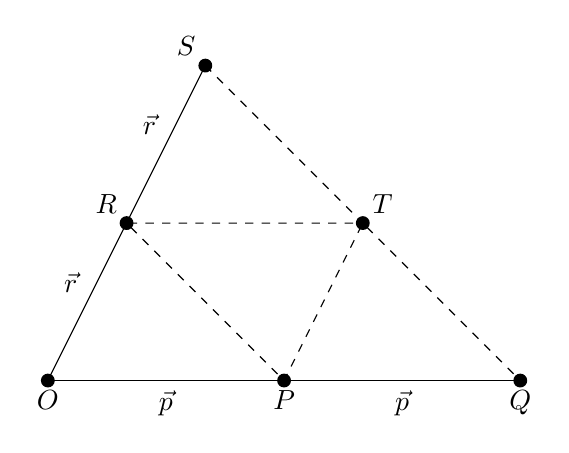
\begin{tikzpicture}
            \coordinate[label=below:$O$] (O) at (0, 0);
            \coordinate[label=below:$P$] (P) at (3, 0);
            \coordinate[label=below:$Q$] (Q) at (6, 0);
            \coordinate[label=above left:$R$] (R) at (1, 2);
            \coordinate[label=above left:$S$] (S) at (2, 4);
            \coordinate[label=above right:$T$] (T) at (4, 2);

            \draw[->] (O) -- (P);
            \draw[->] (P) -- (Q);
            \draw[->] (O) -- (R);
            \draw[->] (R) -- (S);
            \draw[dashed] (S) -- (T) -- (R) -- (P) -- (T) -- (Q);

            \fill (O) circle[radius=2.5pt];
            \fill (P) circle[radius=2.5pt];
            \fill (Q) circle[radius=2.5pt];
            \fill (R) circle[radius=2.5pt];
            \fill (S) circle[radius=2.5pt];
            \fill (T) circle[radius=2.5pt];

            \node[anchor=north] at (1.5, 0) {$\vec p$};
            \node[anchor=north] at (4.5, 0) {$\vec p$};

            \node[anchor=south east] at (0.5, 1) {$\vec r$};
            \node[anchor=south east] at (1.5, 3) {$\vec r$};
        \end{tikzpicture}
    \end{center}
    Clearly, $PRTQ$ is a parallelogram. Likewise, $ORTP$ is also a parallelogram.
\end{solution}

\begin{problem}
    The position vectors of points $A$, $B$, $C$ are given by $\oa{OA} = 5\vec i$, $\oa{OB} = \vec i + 3\vec k$, $\oa{OC} = \vec i + 4\vec j$. A parallelepiped has $OA$, $OB$ and $OC$ as three edges, and the remaining edges are $X$, $Y$, $Z$ and $D$ as shown in the diagram.

    \begin{center}\tikzsetnextfilename{338}
        \begin{tikzpicture}
            \coordinate[label=below:$A$] (A) at (5, 0);
            \coordinate[label=left:$B$] (B) at (1, 3);
            \coordinate[label=left:$C$] (C) at (2, 2);
            \coordinate[label=above:$D$] (D) at (8, 5);
            \coordinate[label=above:$X$] (X) at (3, 5);
            \coordinate[label=right:$Y$] (Y) at (7, 2);
            \coordinate[label=above left:$Z$] (Z) at (6, 3);
            \coordinate[label=below:$O$] (O) at (0, 0);

            \draw (B) -- (O) -- (A) -- (Y) -- (D) -- (X) -- (B) -- (Z) -- (A);
            \draw (Z) -- (D);
            \draw[dotted] (O) -- (C) -- (X);
            \draw[dotted] (C) -- (Y);
        \end{tikzpicture}
    \end{center}

    \begin{enumerate}
        \item Write down the position vectors of $X$, $Y$, $Z$ and $D$ in terms of $\vec i$, $\vec j$ and $\vec k$, and calculate the length of $OD$.
        \item Calculate the size of angle $OZY$.
        \item The point $P$ divides $CZ$ in the ratio $\l : 1$. Write down the position vector of $P$, and evaluate $\l$ if $\oa{OP}$ is perpendicular to $\oa{CZ}$.
    \end{enumerate}
\end{problem}
\begin{solution}
    \begin{ppart}
        We have
        \begin{alignat*}{2}
            \oa{OX} &= \phantom{\oa{OA} + } \oa{OB} + \oa{OC} &&= 2\vec i + 4\vec j + 3\vec k,\\
            \oa{OY} &= \oa{OA} \phantom{+ \oa{OB}} + \oa{OC} &&= 6\vec i + 4\vec j,\\
            \oa{OZ} &= \oa{OA} + \oa{OB} \phantom{+ \oa{OC}} &&= 6\vec i + 3\vec k,\\
            \oa{OD} &= \oa{OA} + \oa{OB} + \oa{OC} &&= 7\vec i + 4\vec j + 3\vec k.
        \end{alignat*}
    \end{ppart}
    \begin{ppart}
        Note that $\oa{ZY} = \cveciiix04{-3}$. Hence, \[\cos \angle OZY = \frac{\oa{OZ} \dotp \oa{ZY}}{\abs{\oa{OZ}} \abs{\oa{ZY}}} = \frac{9}{\sqrt{45} \sqrt{25}} \implies \angle OZY = 74.4\deg \todp{1}.\]
    \end{ppart}
    \begin{ppart}
        By the ratio theorem, \[\oa{OP} = \frac{\oa{OC} + \l \oa{OZ}}{1 + \l} = \frac1{1 + \l} \bs{3\l\cveciii201 + \cveciii140}.\] Note that $\oa{CZ} = \cveciiix5{-4}{3}$. Since $\oa{OP} \perp \oa{CZ}$, we have \[\oa{OP} \dotp \oa{CZ} = 0.\] Hence, \[3\l\cveciii201 \dotp \cveciii5{-4}{3} + \cveciii140 \dotp \cveciii5{-4}{3} = 39 \l - 11= 0,\] whence $\l = 11/39$.
    \end{ppart}
\end{solution}

\begin{problem}
    The vectors $\vec a$, $\vec b$ and $\vec c$ are such that $\vec a \dotp \vec b = \vec b \dotp \vec c = 0$ and $\vec a \dotp \vec c = 2$. Given that $\abs{\vec a} = 1$, $\abs{\vec b} = 2$, $\abs{\vec c} = 3$, find
    \begin{enumerate}
        \item $\abs{\vec a - \vec b}$;
        \item $\abs{\vec a - \vec b - \vec c}$.
    \end{enumerate}
\end{problem}
\begin{solution}
    \begin{ppart}
        Observe that \[\abs{\vec a - \vec b}^2 = \bp{\vec a - \vec b} \dotp \bp{\vec a - \vec b} = \vec a \dotp \vec a - \vec a \dotp \vec b - \vec b \dotp \vec a + \vec b \dotp \vec b.\] Since  $\vec a \dotp \vec b = 0$, we get \[\abs{\vec a - \vec b}^2 = \vec a \dotp \vec a + \vec b \dotp \vec b = \abs{\vec a}^2 + \abs{\vec b}^2 = 1^1 + 2^2 = 5.\] Thus, $\abs{\vec a - \vec b} = \sqrt5$.
    \end{ppart}
    \begin{ppart}
        Observe that \[\abs{\vec a- \vec b - \vec c}^2 = \bp{\vec a - \vec b - \vec c}\dotp \bp{\vec a - \vec b - \vec c} = \bp{\vec a - \vec b} \dotp \bp{\vec a - \vec b} - 2\vec c \dotp \bp{\vec a - \vec b} + \vec c \dotp \vec c.\] Since $\vec a \dotp \vec c = 2$ and $\vec b \dotp \vec c = 0$, we have \[\abs{\vec a- \vec b - \vec c}^2 = \abs{\vec a - \vec b}^2 -2(2) + \abs{\vec c}^2 = 5 - 2(2) + 3^2 = 10.\] Thus, $\abs{\vec a - \vec b - \vec c} = \sqrt{10}$.
    \end{ppart}
\end{solution}

\begin{problem}
    The position vectors of the points $M$ and $N$ are given by \[\oa{OM} = \l \vec i + (2\l - 1) \vec j + \vec k, \qquad \oa{ON} = (1-\l) \vec i + 3\l \vec j - 2 \vec k,\] where $\l$ is a scalar. Find the values of $\l$ for which $\oa{OM}$ and $\oa{ON}$ are perpendicular. When $\l = 1$, find the size of $\angle MNO$ to the nearest degree.
\end{problem}
\begin{solution}
    Since $\oa{OM} \perp \oa{ON}$, we have \[\oa{OM} \dotp \oa{ON} = \cveciii{\l}{2\l - 1}{1} \dotp \cveciii{1-\l}{3\l}{-2} = 5\l^2 - 2\l -2 = 0.\] Solving the quadratic, we get \[\l = \frac{1 \pm \sqrt{11}}{5}.\]

    When $\l = 1$, we have \[\oa{OM} = \cveciii111, \quad \oa{ON} = \cveciii03{-2}, \quad \oa{MN} = \cveciii{-1}2{-3}.\] Hence, \[\cos \angle MNO = \frac{\oa{ON} \dotp \oa{MN}}{\abs{\oa{ON}} \abs{\oa{MN}}} = \frac{12}{\sqrt{13} \sqrt{14}} \implies \angle MNO = 27\deg.\]
\end{solution}

\begin{problem}
    The points $A$, $B$, $C$ and $D$ have position vectors $\vec i - 2\vec j + 5\vec k$, $\vec i + 3\vec j$, $10\vec i + \vec j + 2\vec k$ and $-2\vec i + 4\vec j + 5\vec k$ respectively, with respect to an origin $O$. The point $P$ on $AB$ is such that $AP : PB = \l : 1 - \l$ and point $Q$ on $CD$ is such that $CQ : QD = \m : 1 - \m$. Find $\oa{OP}$ and $\oa{OQ}$ in terms of $\l$ and $\m$ respectively.

    Given that $PQ$ is perpendicular to both $AB$ and $CD$, show that $\oa{PQ} = \vec i + 2\vec j + 2\vec k$.
\end{problem}
\begin{solution}
    By the ratio theorem, \[\oa{OP} = \frac{(1 - \l) \oa{OA} + \l \oa{OB}}{(1 - \l) + \l} = \oa{OA} + \l \bp{\oa{OB} - \oa{OA}} = \cveciii1{-2}5 + 5\l \cveciii01{-1}\] and \[\oa{OQ} = \frac{(1-\m) \oa{OC} + \oa{OD}}{(1-\m) + \m} = \oa{OC} + \m \bp{\oa{OD} - \oa{OC}} = \cveciii{10}{1}{2} + 3\m \cveciii{-4}{1}{1}.\]

    Note that \[\oa{PQ} = \bs{\cveciii{10}{1}{2} + 3\m \cveciii{-4}{1}{1}} - \bs{\cveciii1{-2}5 + 5\l \cveciii01{-1}} = 3\cveciii31{-1} + 3\m \cveciii{-4}11 - 5\l \cveciii01{01}.\]

    Since $PQ$ is perpendicular to $AB$, we have \[\oa{PQ} \dotp \oa{AB} = \bs{3\cveciii31{-1} + 3\m \cveciii{-4}11 - 5\l \cveciii01{01}} \dotp \bs{5\cveciii01{-1}} = 5(6 -10 \l) = 0.\] Thus, $\l = 3/5$.

    Since $PQ$ is perpendicular to $CD$, we have \[\oa{PQ} \dotp \oa{CD} = \bs{3\cveciii31{-1} + 3\m \cveciii{-4}11 - 5\l \cveciii01{01}} \dotp \bs{3\cveciii{-4}11} = 3(-36 + 54\m) = 0.\] Thus, $\m = 2/3$.

    Hence, \[\oa{PQ} = 3\cveciii31{-1} + 3\bp{\frac23} \cveciii{-4}11 - 5\bp{\frac35} \cveciii01{-1} = \cveciii122.\]
\end{solution}

\begin{problem}
    The position vectors of the vertices $A$, $B$ and $C$ of a triangle are $\vec a$, $\vec b$ and $\vec c$ respectively. If $O$ is the origin and not within the triangle, show that the area of triangle $OAB$ is $\frac12 \abs{\vec a \crossp \vec b}$, and deduce and expression for the area of the triangle $ABC$.

    Hence, or otherwise, show that the perpendicular distance from $B$ to $AC$ is \[\frac{\abs{\vec a \crossp \vec b + \vec b \crossp \vec c + \vec c \crossp \vec a}}{\abs{\vec c - \vec a}}.\]
\end{problem}
\begin{solution}
    Let $\t = \angle AOB$ be the angle between $\vec a$ and $\vec b$. Clearly, \[[\triangle OAB] = \frac12 (OA) (OB) \sin \t = \frac12 \abs{\vec a \crossp \vec b}.\]

    Note that $AB = \abs{\vec b - \vec a}$ and $AC = \abs{\vec c - \vec a}$. Hence, \[[\triangle ABC] = \frac12 \abs{(\vec b - \vec a) \crossp \vec (\vec c - \vec a)}.\] Expanding, we get \[[\triangle ABC] = \frac12 \abs{\vec b \crossp \vec c - \vec b \crossp \vec a - \vec a \crossp \vec c} = \frac12 \abs{\vec a \crossp \vec b + \vec b \crossp \vec c + \vec c \crossp \vec a}.\]

    Let the perpendicular distance from $B$ to $AC$ be $h$. Then \[[\triangle ABC] = \frac12 h (AC) = \frac12 h \abs{\vec c - \vec a}.\] Hence, \[h = \frac{2 [\triangle ABC]}{\abs{\vec c- \vec a}} = \frac{\abs{\vec a \crossp \vec b + \vec b \crossp \vec c + \vec c \crossp \vec a}}{\abs{\vec c - \vec a}}.\]
\end{solution}

\begin{problem}[\chili]
    The points $A$, $B$ and $C$ lie on a circle with centre $O$ and diameter $AC$. It is given that $\oa{OA} = \vec a$ and $\oa{OB} = \vec b$.

    \begin{enumerate}
        \item Find $\oa{BC}$ in terms of $\vec a$ and $\vec b$. Hence, show that $AB$ is perpendicular to $BC$.
        \item Given that $\angle AOB = 30\deg$, find $\oa{OF}$ where $F$ is the foot of perpendicular of $B$ to $AC$. Hence, find $\oa{OB'}$, where $B'$ is the reflection of $B$ in the line $AC$.
    \end{enumerate}
\end{problem}
\begin{solution}
    \begin{ppart}
        Since $A$, $B$ and $C$ lie on the same circle, $\abs{\vec a} = \abs{\vec b} = \abs{\vec c}$. Since $AC$ is the diameter of the circle, $\vec c$ is in the opposite direction as $\vec a$. Hence, $\vec c = -\vec a$. Thus, \[\oa{BC} = \oa{OC} - \oa{OB} = -\vec a- \vec b.\] Also note that \[\oa{AB} = \oa{OB} - \oa{OA} = \vec b - \vec a.\] Consider $\oa{AB} \dotp \oa{BC}$: \[\oa{AB} \dotp \oa{BC} = \bp{\vec b - \vec a} \dotp -\bp{\vec a + \vec b} = -\bp{\vec b \dotp \vec b - \vec a \dotp \vec a} = -\bp{\abs{\vec b}^2 - \abs{\vec a}^2} = 0.\] Thus, $AB$ is perpendicular to $BC$.
    \end{ppart}
    \begin{ppart}
        Observe that \[\frac{\sqrt3}{2} = \cos \angle AOB = \frac{OF}{OB} = \frac{\abs{\oa{OF}}}{\abs{\vec a}} \implies \abs{\oa{OF}} = \frac{\sqrt{3}}{2} \abs{\vec a}.\] Since $\oa{OF}$ is in the same direction as $\oa{OA}$, we have \[\oa{OF} = \frac{\sqrt3}{2} \vec a.\]

        Note that \[\oa{BF} = \frac{\sqrt3}2 \vec a - \vec b.\] By the midpoint theorem, \[\oa{OF} = \frac{\oa{OB} + \oa{OB'}}{2} \implies \oa{OB'} = 2\oa{OF} - \oa{OB} = \sqrt{3} \vec a - \vec b.\]
    \end{ppart}
\end{solution}